%%%%%%%%%%%%%%%%%%%%%%%%%%%%%%%%%%%%%%%%%%%%%%%%%%%%%%%%%%%%%%%%
% %
% Due Date %
% Andrew Gibson %
% ECE 351 lab, Section 53 %
% Lab 11 %
% Due 11 Apr 2023 %
% Z - Transform Operations %
% https://github.com/gibs0630/ECE351\_Code %
% https://github.com/gibs0630/ECE351\_Reports %
% %
%%%%%%%%%%%%%%%%%%%%%%%%%%%%%%%%%%%%%%%%%%%%%%%%%%%%%%%%%%%%%%%%

\documentclass[12pt,a4paper]{article}
\usepackage[utf8]{inputenc}
\usepackage[greek,english]{babel}
\usepackage{alphabeta} 
\usepackage[pdftex]{graphicx}
\usepackage[top=1in, bottom=1in, left=1in, right=1in]{geometry}
\linespread{1.06}
\setlength{\parskip}{8pt plus2pt minus2pt}
\widowpenalty 10000
\clubpenalty 10000
\newcommand{\eat}[1]{}
\newcommand{\HRule}{\rule{\linewidth}{0.5mm}}
\usepackage[official]{eurosym}
\usepackage{enumitem}
\setlist{nolistsep,noitemsep}
\usepackage[hidelinks]{hyperref}
\usepackage{cite}
\usepackage{lipsum}

\newcommand{\Q}{\leavevmode\par\textbf {Q:}}
\newcommand{\A}{\par\textbf{A:} \normalfont}

\hypersetup{colorlinks=true, linkcolor=black, urlcolor=blue}

\begin{document}
%===========================================================
\begin{titlepage}
\begin{center}
% Top 
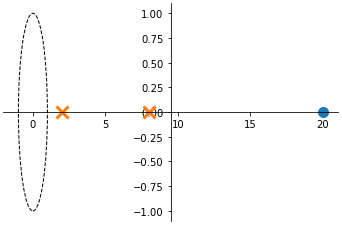
\includegraphics[width=0.55\textwidth]{titlepage_image.png}~\\[2cm]
% Title
\HRule \\[0.4cm]
{ \LARGE 
  \textbf{Project Report for ECE 351}\\[0.4cm]
  \emph{Lab 11: Z - Transform Operations}\\[0.4cm]
}
\HRule \\[1.5cm]
% Author
{ \large
  Andrew Gibson \\[0.1cm]
 4 April 2023\\[0.1cm]
  \url{https://github.com/gibs0630/ECE351\_Code}\\[0.1cm]
  \url{https://github.com/gibs0630/ECE351\_Reports}\\[0.1cm]
  %#\texttt{user@cut.ac.cy}
}
\vfill
%\textsc{\Large Cyprus University of Technology}\\[0.4cm]\textsc{\large Department of Electrical Engineering,\\Computer Engineering \& Informatics}\\[0.4cm]
% Bottom
{\large }
 
\end{center}
\end{titlepage}
%\begin{abstract}
%\lipsum[1-2]
%\addtocontents{toc}{\protect\thispagestyle{empty}}
%\end{abstract}
\newpage
%===========================================================
\tableofcontents
\addtocontents{toc}{\protect\thispagestyle{empty}}
\newpage
\setcounter{page}{1}
%===========================================================
%===========================================================
\section{Introduction}\label{sec:intro}
With Python, it is possible to easily compute properties of a z-transformed  function.

\section{Equations}\label{sec:lit-rev}


equations from the lab
\[y[k] = 2 x[k] - 40 x[k-1] + 10 y[k-1] - 16 y[k-2]\]


\section{Methodology}\label{sec:meth}
This lab had us compute the transfer function in the time domain and z domain. Python was then used to extrapolate additional information, such as stability, or gain for a given frequency.

\section{Results}\label{sec:res}
\subsection*{task 1}
\[y[k] = 2 x[k] - 40 x[k-1] + 10 y[k-1] - 16 y[k-2]\]

y[k] is causal, so both the left hand side and right hand side are multiplied by u[k]

\[Y[z] = 2 X[z] - 40 (z^{-1} X[k] + x[-1]) + 10 (z^{-1} Y[k] + y[-1])-16 (z^{-2} Y[k] + z^-1 y[-1]+ y[-2])\]

\[Y[z] = 2 X[z] - 40 (z^{-1} X[k] + (0)) + 10 (z^{-1} Y[k] + (0)) - 16 (z^{-2} Y[k] + z^{-1} (0) + (0))\]

\[Y[z] = 2 X[z] - 40(z^{-1} X[k] + 10 z^{-1} Y[k] - 16 z^{-2} Y[k]\]

\[16 z^{-2} Y[k] - 10 z^{-1} Y[k] + Y[z] = 2 X[z] - 40 z^{-1} X[k]\]

\[(16 z^{-2} - 10 z^{-1} + 1) Y[z] = (2 - 40 z^{-1}) X[k]\]

\[\frac{Y[z]}{X[k]} = \frac{2 - 40 z^{-1}}{16 z^{-2} - 10 z^{-1} + 1}\]

\[H[k] = \frac {2 - 40 z^{-1}}{16 z^{-2} - 10 z^-{1} + 1}\]

\[H[k] = \frac{2 z^2 - 40 z^1}{16 - 10 z^1 + 1z^2}\]

\[H[k] = \frac{2 z^2 - 40 z}{z^2-10 z^1+16}\]


\subsection*{task 2}

\[\frac{H[k]}{z} = \frac{2 z - 40}{z^2 - 10 z^1 + 16}\]

\[\frac{2 z - 40}{(z-8)(z-2)} = \frac {A}  {(z-8)} + \frac{B}{(z-2)}\]

\[A = \frac{2 z - 40} {z-2} \Bigg|_{z = 8}  \]

\[A = -4\]

\[B = \frac{2 z - 40}{z-8} \Bigg|_{z = 2}  \]

\[B = 6\]


\[\frac{H[k]}{z} = \frac{-4} {z-8} + \frac {6}{z-2}\]

\[H[k] = \frac{-4 z}{z-8} + \frac{6 z}{z-2}\]

\[H[k] = \frac{-4 z}{z-8} + \frac{6 z}{z-2}\]


\[h[k] = (-4) 8^k u[k]+ (6) 2^k u[k]\]

\subsection*{task 3}

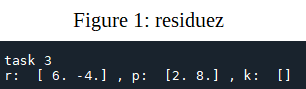
\includegraphics[width=0.5\textwidth]{Figure 1.png}\\
Figure 1 shows the residue (aka zeroes), poles, and stand alone coefficients using the scipy.signal.residuez function \\


\subsection*{task 4}
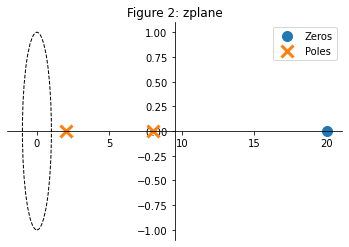
\includegraphics[width=0.8\textwidth]{Figure 2.png}\\
Figure 2 shows the plot of complex z - plane given a transfer function.  If the poles are within the unit circle (dashed oval) then the function is stable.  if there is a mix of poles inside and outside the unit circle, then L'Hospital rule may have to be used.\\


\subsection*{task 5}
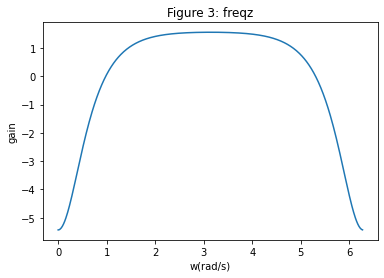
\includegraphics[width=0.8\textwidth]{Figure 3.png}\\
Figure 3 the gain for a given frequency using the scipy.signal.freqz function.\\


\section{Questions}\label{sec:res}

\Q Looking at the plot generated in Task 4, is H(z) stable? Explain why or why not.
\A zeroes have no effect on stability, so we can ignore the zero at 20
 Sue to the relation $\mathcal{Z}\{a^k u[k]\} = \frac{z}{(z-a)}$, then if $a$ is is less then one, then it is stable. looking at the plot, there are two poles, and both are outside the unit circle, thus this . This would be causal function would be unstable.

\Q Leave any feedback on the clarity of lab tasks, expectations, and deliverables
\A the poles and zeroes plot was new, perhaps an explanation of what it is prior to the lab would be helpful for future classes.



%\lipsum[7-8]\cite{knuthwebsite}
%===========================================================
%===========================================================
\bibliographystyle{ieeetr}
\bibliography{refs}
\end{document} 
Annotations











